\section{Testaufbau im Labor der FHNW}
Wie in Kapitel \ref{chptr:_einleitung} erwähnt wurde ein Testaufbau im Labor der FHNW aufgebaut, auf der die Steuerung getestet werden soll. Auf der Abb. \ref{fig:testaufbau} sind die Halterung für die Pumpdiode, die Kollimierungslinsen für das Richten des Laserstrahls und die Kristallhalterung zu sehen. Für eine verbesserte Wärmeleitung wird einen Wärmeleitpaste auf die Flächen des TECs aufgetragen.

Für die Wasserkühlung wurde die Pumpdiodenhalterung für die Pumpdiode im Rahmen des Projektes ebenfalls erstellt. Das Schema ist im Anhang unter dem Kapitel \ref{chptr:_pumpdiodenhalterung} enthalten. Im Rahmen dieser Arbeit wird jedoch nicht weiter auf die Halterung eingegangen.

\begin{figure}[H]
    \centering
    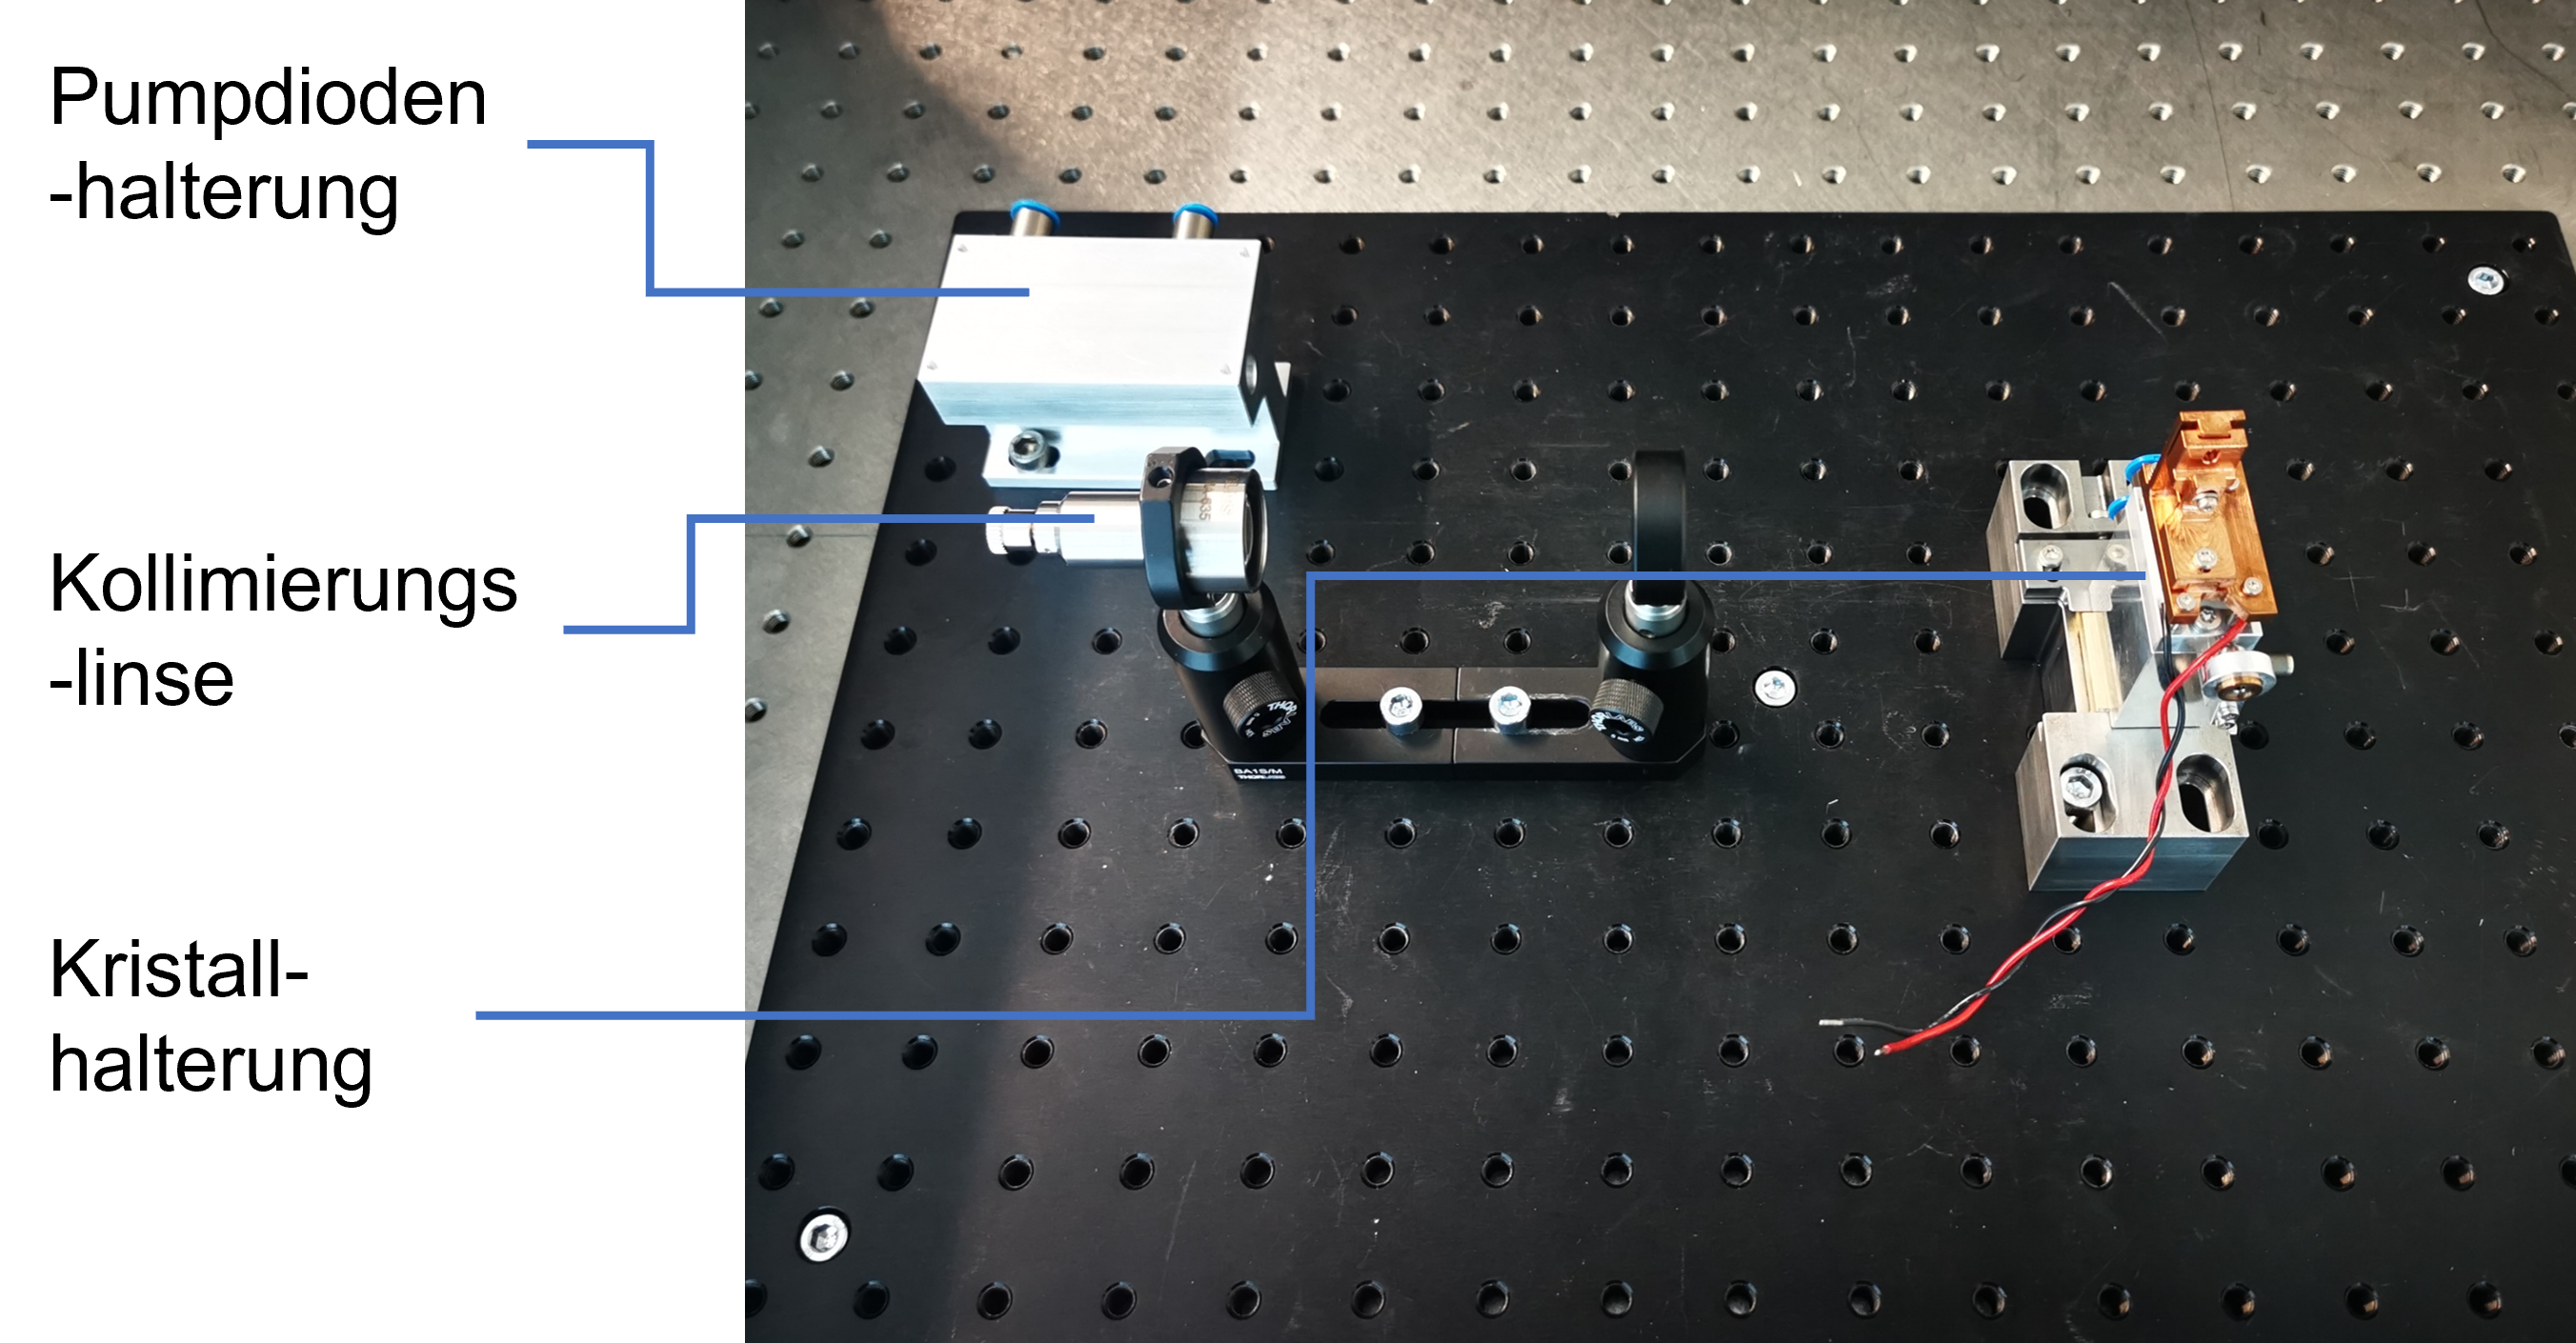
\includegraphics[scale=0.6]{98_images/testaufbau.png}
    \caption{Der Testaufbau, wie dieser im Labor der FHNW vorbereitet wurde.}
    \label{fig:testaufbau}
\end{figure}